\documentclass[a4paper]{article}
\usepackage[utf8]{inputenc}


%=-=-=-=-=-=-=-=-=-=-=-=-=-=-=-=-=-=-=-=-=-=-=-=-=-=-=-=-=-=-=-=-=-=-=-=-=-=-=-=-
% PREAMBLE
%=-=-=-=-=-=-=-=-=-=-=-=-=-=-=-=-=-=-=-=-=-=-=-=-=-=-=-=-=-=-=-=-=-=-=-=-=-=-=-=-

%%%%%%%%%%%%%%%%%%%%%%%%%%%%%%%%%%%%%%%%%%%%%%%%%%%%%%%%%%%%%%%%%%%%%
% Important styling notes
%%
% For now, to include img.jpg in img/path/to/img.jpg, just use:
% path/to/img.jpg - for details see style.tex
%=-=-=-=-=-=-=-=-=-=-=-=-=-=-=-=-=-=-=-=-=-=-=-=-=-=-=-=-=-=-=-=-=-=-=-=-=-=-=-=-
% Packages
%%
%\usepackage{fullpage} % Package to use full page
\usepackage[top=1in,bottom=1in,left=1in,right=0.7in,heightrounded]{geometry}

\usepackage{parskip}                    % Package to tweak paragraph skipping
\usepackage{amsmath}                    % standard
\usepackage{amssymb}                    % standard - Double R symbol etc.
\usepackage{hyperref}
\usepackage{amsthm}                     % standard - theorem, definition, etc.
\usepackage{multicol}                   % multiple columns for numbering
\usepackage{enumitem}                   % standard - enumerate styles
\usepackage[utf8]{inputenc}
\usepackage{scrextend}                  % indentation
\usepackage{graphicx}                   % standard - add figures
\usepackage{float}                      % standard - figure position, use [H] option
\usepackage{pifont}                     % symbols
\usepackage{gensymb}                    % degree symbol \degree
\usepackage{xcolor}                     % bg color
\hypersetup{
    colorlinks,
    linkcolor={black!50!black},
    citecolor={blue!50!black},
    urlcolor={blue!80!black}
}
\usepackage{framed}                     % bg color
\usepackage[T1]{fontenc}                % small caps
\usepackage{sectsty}                    % headings colour
\usepackage{mathtools}                  % Loads amsmath
\usepackage{amsthm,thmtools,xcolor}     % coloured theorem
\usepackage[toc,page]{appendix}         % reference to appendix
%\usepackage{titlesec}                   % change chapter, section, etc. formats
\usepackage{xifthen}                    % if, else
\usepackage{etoolbox}
% format numbering in theorem, lemma, etc. environment
\AtBeginEnvironment{theorem}{\setlist[enumerate, 1]{font=\upshape,  wide=0.5em, before=\leavevmode}}
\AtBeginEnvironment{lemma}{\setlist[enumerate, 1]{font=\upshape,  wide=0.5em, before=\leavevmode}}
\usepackage[letterspace=150]{microtype} % \textls{<letterspaced text>} % 0 <= letterspace <= 1000, 1000 = M space
\usepackage{letltxmacro}                % renew commands?
\usepackage{minted}                     % package to list code
    % otherwise minted goes off the page
    \setmintedinline{breaklines}
\usepackage{subfig}
\usepackage{eso-pic}                    % title page bg pic
\usepackage{varwidth}
\PassOptionsToPackage{svgnames}{xcolor}
\usepackage{fontawesome}                % \faQuestionCircle
\usepackage{marvosym}                   %\Pointinghand
\usepackage{mdframed}                   % easy outline frames
\usepackage[many]{tcolorbox}            % colour box for theorem styles
\usepackage{array,booktabs,calc} % table figs and text
\usepackage{comment}                    % \begin{comment}
\usepackage{fancyhdr}                   % page headings
\usepackage{mdframed}                   % boxes
\usepackage[backend=biber,sorting=none,style=ieee]{biblatex}
\usepackage{caption}
%%% caption options {
%\DeclareCaptionFont{white}{\color{white}}
\DeclareCaptionFormat{listing}{\colorbox{magenta!30!gray}{\parbox{\textwidth}{#1#2#3}}}
\captionsetup[lstlisting]{format=listing,labelfont={bf,small},textfont=small,skip=-1pt}
%%% }
\addbibresource{bibliography.bib}
\usepackage{url}
\usepackage{textcomp}
\usepackage[makeroom]{cancel}            % crossed symbols
\usepackage{algorithm}
\usepackage[noend]{algpseudocode}
\usepackage{tikz}
\usetikzlibrary{arrows.meta,positioning,quotes} % arrows and nodes in tikz
\usepackage{marginnote}
\usepackage{pgfplots}
\usepackage{pstricks-add,pst-slpe}  % for fancy tikz arrows
%\usepackage{titlesec}                   % title style
\usepackage{lmodern}                    % a font
\usepackage{titletoc} % Required for manipulating the table of contents
\usepackage{titlesec} % Allows customization of titles
\usepackage{fouriernc} % Use the New Century Schoolbook font
\usepackage{booktabs} % things in page margins
\usepackage{stmaryrd } % \varoast
\usepackage{listings} % code listings
\usepackage{longtable} % table across multiple pages
\usepackage{styles/nasm/lang}  % include custom language for NASM assembly.
\usepackage{styles/nasm/style} % include custom style for NASM assembly.



%% extra comments that I don't know where they belong:
% list of ding tags: http://willbenton.com/wb-images/pifont.pdf

%=-=-=-=-=-=-=-=-=-=-=-=-=-=-=-=-=-=-=-=-=-=-=-=-=-=-=-=-=-=-=-=-=-=-=-=-=-=-=-=-
% Colours for various things
%%


\definecolor{shadecolor}{rgb}{1.,0.933,0.96} % bg color, r,g,b <= 1
\definecolor{medium_blue}{RGB}{60,125,190}
\definecolor{dark_blue}{RGB}{25,60,85}
\definecolor{dark_red}{RGB}{77,16,16}
\definecolor{LightPink}{rgb}{0.92.,0.8,0.84} % bg color, r,g,b <= 1
\definecolor{LighterPink}{rgb}{1.,0.94,0.97} % bg color, r,g,b <= 1
\definecolor{LightestPink}{rgb}{1.,0.95,0.99} % bg color, r,g,b <= 1
\definecolor{DarkestPink}{rgb}{0.36, 0.0, 0.18}
\definecolor{DarkerPink}{rgb}{0.41, 0.0, 0.21}
\definecolor{DarkPink}{rgb}{0.55, 0.05, 0.37}
\definecolor{lightestestpink}{RGB}{255,248,252}
\definecolor{codegray}{rgb}{0.5,0.5,0.5}
\definecolor{codegrayblue}{rgb}{0.35,0.35,0.47}



%=-=-=-=-=-=-=-=-=-=-=-=-=-=-=-=-=-=-=-=-=-=-=-=-=-=-=-=-=-=-=-=-=-=-=-=-=-=-=-=-
% Define my own theorem styles
%%

% "base" styles
\declaretheoremstyle[
  headfont=\color{DarkPink}\bfseries,
  bodyfont=\itshape,
]{colored}

\declaretheoremstyle[
  headfont=\color{DarkPink}\bfseries,
  bodyfont=\normalfont,
]{colored_upright}

% theorems (corollaries, etc) themselves, inherit from my style above
% Usage:
% \begin{theorem} \end{theorem}, \begin{lemma} \end{lemma}, ...
\declaretheorem[
	numberwithin=section,
 	style=colored,
	name=\textsc{Theorem},
]{theorem}

\tcolorboxenvironment{theorem}{
  boxrule=0pt,
  boxsep=2pt,
  colback={magenta!25!white},
  colframe=DarkPink,
  enhanced jigsaw, 
  borderline west={2pt}{0pt}{DarkPink},
  sharp corners,
  before skip=5pt,
  after skip=5pt,
  breakable,
  right=0mm % for equations
}

\declaretheorem[
	numberwithin=section,
 	style=colored,
	name=\textsc{Corollary},
]{corollary}

\tcolorboxenvironment{corollary}{
  boxrule=0pt,
  boxsep=1pt,
  colback={magenta!10!white},
  colframe=DarkPink,
  enhanced jigsaw, 
  borderline west={2pt}{0pt}{DarkPink},
  sharp corners,
  before skip=5pt,
  after skip=5pt,
  breakable,
  right=0mm % for equations
}

\declaretheorem[
	numberwithin=section,
	style=colored,
	name=\textsc{Lemma},
]{lemma}

\tcolorboxenvironment{lemma}{
  boxrule=0pt,
  boxsep=1pt,
  colback={magenta!10!white},
  colframe=DarkPink,
  enhanced jigsaw, 
  borderline west={2pt}{0pt}{DarkPink},
  sharp corners,
  before skip=5pt,
  after skip=5pt,
  breakable,
  right=0mm % for equations
}

\declaretheorem[
	numberwithin=section,
	style=colored,
	name=\textsc{Definition},
]{definition}

\tcolorboxenvironment{definition}{
  boxrule=0pt,
  boxsep=1pt,
  colback={magenta!25!white},
  colframe=DarkPink,
  enhanced jigsaw, 
  borderline west={2pt}{0pt}{DarkPink},
  sharp corners,
  before skip=5pt,
  after skip=5pt,
  breakable,
  right=0mm % for equations
}

\declaretheorem[
	numberwithin=section,
  	style=colored,
  	name=\textsc{Example},
]{exmp}

\declaretheorem[
	numberwithin=section,
  	style=colored,
  	name=\textsc{Solution},
]{soln}

%%% code listings
\lstdefinestyle{code1}{
    backgroundcolor=\color{lightestestpink},   
    commentstyle=\color{codegrayblue},
    keywordstyle=\color{DarkerPink},
    numberstyle=\tiny\color{codegray},
    stringstyle=\color{black!40!cyan},
    basicstyle=\small\ttfamily,
    breakatwhitespace=false,
    breaklines=true,        
    captionpos=t,             
    keepspaces=true,        
    numbers=left,           
    numbersep=5pt,
    showspaces=false, 
    showstringspaces=false,
    showtabs=false,
    tabsize=4
}

\lstset{style=code1}

%=-=-=-=-=-=-=-=-=-=-=-=-=-=-=-=-=-=-=-=-=-=-=-=-=-=-=-=-=-=-=-=-=-=-=-=-=-=-=-=-
% Headers (size, font, colour)
%%




\makeatletter
\renewcommand{\@seccntformat}[1]{\llap{\textcolor{DarkestPink}{\csname the#1\endcsname}\hspace{1em}}}                    
\renewcommand{\section}{\@startsection{section}{1}{\z@}
{-4ex \@plus -1ex \@minus -.4ex}
{1ex \@plus.2ex }
{\normalfont\large\sffamily\bfseries\textcolor{DarkestPink}}}
\renewcommand{\subsection}{\@startsection {subsection}{2}{\z@}
{-3ex \@plus -0.1ex \@minus -.4ex}
{0.5ex \@plus.2ex }
{\normalfont\sffamily\bfseries\textcolor{DarkestPink}}}
\renewcommand{\subsubsection}{\@startsection {subsubsection}{3}{\z@}
{-2ex \@plus -0.1ex \@minus -.2ex}
{.2ex \@plus.2ex }
{\normalfont\small\sffamily\bfseries\textcolor{DarkestPink}}}                        


%=-=-=-=-=-=-=-=-=-=-=-=-=-=-=-=-=-=-=-=-=-=-=-=-=-=-=-=-=-=-=-=-=-=-=-=-=-=-=-=-
% Numberings, counters and spacings
%%
\numberwithin{equation}{section} % section number in eq/s
\setlength{\jot}{7pt} % spacing in split, gathered env/s



%% Custom examples
%% Output - Example 1,2,...
\newcounter{example}
\newenvironment{example}[1][]{\refstepcounter{example}\par\medskip
   \textbf{Example~\theexample. #1} \rmfamily}{\medskip}
%%%%%%%%%%%% End of unused %%%%%%%%%%%%



%=-=-=-=-=-=-=-=-=-=-=-=-=-=-=-=-=-=-=-=-=-=-=-=-=-=-=-=-=-=-=-=-=-=-=-=-=-=-=-=-
% Paths
%%
\graphicspath{ {./img/} } % figures' path - can look up files directly from there


%=-=-=-=-=-=-=-=-=-=-=-=-=-=-=-=-=-=-=-=-=-=-=-=-=-=-=-=-=-=-=-=-=-=-=-=-=-=-=-=-
% User defined macros (math mode)
%%


% Curly braces under text. Usage: \myunderbrace{upper}{lower}
\newcommand{\myunderbrace}[2]{\mathrlap{\underbrace{\phantom{#1}}_{#2}} #1}
\newcommand{\setR}{\mathbb{R}} % \ouble R
\newcommand{\setRn}{\mathbb{R}^n} %  double R^n
\newcommand{\setN}{\mathbb{N}} % double N
\newcommand{\setZ}{\mathbb{Z}} % double Z
\let\oldemptyset\emptyset
\let\emptyset\varnothing % nice - looking empty set symbol
\newcommand{\fancyN}{\mathcal{N}} % null space
\newcommand{\fancyR}{\mathcal{R}} % range

\newcommand{\bx}{\textbf{x}}
\newcommand{\by}{\textbf{y}}
\newcommand{\bb}{\textbf{b}}
\newcommand{\bA}{\textbf{A}}
\newcommand{\bB}{\textbf{B}}
\newcommand{\bI}{\textbf{I}}
% double bars as in norm
\newcommand{\norm}[1] {\lVert #1 \rVert} 
\newcommand{\trans}[1]{#1^{\top}}

\newcommand{\mean}[1]{\bar{#1}}
\newcommand{\var}{\sigma^2}

\newcommand{\partdevx}[1]{\frac{\partial #1}{\partial x}}
\newcommand{\partdevxx}[1]{\frac{\partial #1}{\partial x}}
\newcommand{\partdevxn}[1]{\frac{\partial^n #1}{\partial x^n}}
\newcommand{\partdevy}[1]{\frac{\partial #1}{\partial x}}
\newcommand{\partdevyy}[1]{\frac{\partial #1}{\partial y}}
\newcommand{\partdevyn}[1]{\frac{\partial^n #1}{\partial y^n}}

% text above = symbol
\newcommand{\overeq}[1]{\ensuremath{\stackrel{#1}=}} 
\newcommand{\greatersmaller}{%
  \mathrel{\ooalign{\raisebox{.6ex}{$>$}\cr\raisebox{-.6ex}{$<$}}}
} % greater and smaller symbols on top of each other, same line

%=-=-=-=-=-=-=-=-=-=-=-=-=-=-=-=-=-=-=-=-=-=-=-=-=-=-=-=-=-=-=-=-=-=-=-=-=-=-=-=-
% User defined macros (non math)

\newcommand{\qedblack}{$\hfill\blacksquare$} % black square end of line
\newcommand{\qedwhite}{\hfill \ensuremath{\Box}} % white square end of line
\newcommand{\hquad}{\hskip0.5em\relax}% half quad space
%\newcommand{\TODO}{\textcolor{red}{\bf TODO!}\;}

\newcommand{\TODO}[1][]{%
    \ifthenelse{\equal{#1}{}}{\textcolor{red}{\bf TODO!}\;}{\textcolor{red}{\textbf {TODO:} #1}\; }%
}
\newcommand{\B}[1]{\textbf{\textup{#1}}} % bold and upright
\renewcommand{\labelitemi}{\scriptsize$\textcolor{DarkPink}{\blacksquare}$} % itemize - squares instead of bullets
\newcommand{\emphasis}[1]{\textls{#1}}

\LetLtxMacro{\originaleqref}{\eqref}
\renewcommand{\eqref}{Eq.~\originaleqref}
\renewcommand*{\eqref}[1]{Eq.~\originaleqref{#1}}





% background images
%%%%%%%
\newcommand\BackgroundPic{%
\put(0,0){%
\parbox[b][\paperheight]{\paperwidth}{%
\vfill
%\centering

\includegraphics[width=0.125\paperwidth,height=\paperheight,%
]{img/background_02.png}% use ,keepaspectratio
\vfill
}}}
%%%%%%%
% end of background image
%%%%%%%%%%%%%% my own frame
\newmdenv[topline=false,bottomline=false]{leftrightbox}
%%%%%%%%%%%%% end
%%%%%%%%%%%%% my own comment
\newcommand{\mycomment}[1]{\begin{leftrightbox}\Pointinghand~\textbf{Comment:}~#1 \end{leftrightbox}}
%%%%%%%%%%%%% end
% my custom note https://tex.stackexchange.com/questions/301993/create-custom-note-environment-with-tcolorbox
\newmdenv[
    topline=false,
    bottomline=false,
    rightline=false,
    innerrightmargin=0pt
]{siderule}
\newenvironment{mynote}%
    {\begin{siderule}\textbf{\Pointinghand~Note:}}
    {\end{siderule}}
%%%%%%%%%%%%% my own box
\newcommand{\boxone}[1]{\begin{tcolorbox}[colback = LighterPink,colframe=LightPink]
#1
\end{tcolorbox}}
%%%%%%%%%%%%% end

\let\oldemptyset\emptyset
\let\emptyset\varnothing
%algorithmic
\algdef{SE}[DOWHILE]{Do}{doWhile}{\algorithmicdo}[1]{\algorithmicwhile\ #1}%






\begin{document}
%=-=-=-=-=-=-=-=-=-=-=-=-=-=-=-=-=-=-=-=-=-=-=-=-=-=-=-=-=-=-=-=-=-=-=-=-=-=-=-=-
% GLOBAL STYLES (DOCUMENT SCOPE)
%=-=-=-=-=-=-=-=-=-=-=-=-=-=-=-=-=-=-=-=-=-=-=-=-=-=-=-=-=-=-=-=-=-=-=-=-=-=-=-=-
% caption: Figure 1 -> <bold> Fig. 1 </bold>
\captionsetup[figure]{labelfont={bf},labelformat={default},labelsep=period,name={Fig.}}


%=-=-=-=-=-=-=-=-=-=-=-=-=-=-=-=-=-=-=-=-=-=-=-=-=-=-=-=-=-=-=-=-=-=-=-=-=-=-=-=-
% TITLE PAGE
%=-=-=-=-=-=-=-=-=-=-=-=-=-=-=-=-=-=-=-=-=-=-=-=-=-=-=-=-=-=-=-=-=-=-=-=-=-=-=-=-
%%%%%%%%%%%%%%%%%%%%%%%%%%%%%%%%%%%%%%%%%
% Formal Book Title Page
% LaTeX Template
% Version 2.0 (23/7/17)
%
% This template was downloaded from:
% http://www.LaTeXTemplates.com
%
% Original author:
% Peter Wilson (herries.press@earthlink.net) with modifications by:
% Vel (vel@latextemplates.com)
%
% License:
% CC BY-NC-SA 3.0 (http://creativecommons.org/licenses/by-nc-sa/3.0/)
% 
% This template can be used in one of two ways:
%
% 1) Content can be added at the end of this file just before the \end{document}
% to use this title page as the starting point for your document.
%
% 2) Alternatively, if you already have a document which you wish to add this
% title page to, copy everything between the \begin{document} and
% \end{document} and paste it where you would like the title page in your
% document. You will then need to insert the packages and document 
% configurations into your document carefully making sure you are not loading
% the same package twice and that there are no clashes.
%
%%%%%%%%%%%%%%%%%%%%%%%%%%%%%%%%%%%%%%%%%

%----------------------------------------------------------------------------------------
%	PACKAGES AND OTHER DOCUMENT CONFIGURATIONS
%----------------------------------------------------------------------------------------



%----------------------------------------------------------------------------------------
%	TITLE PAGE
%----------------------------------------------------------------------------------------



\begin{titlepage} % Suppresses headers and footers on the title page

	\centering % Centre everything on the title page
	
	\scshape % Use small caps for all text on the title page
	
	\vspace*{\baselineskip} % White space at the top of the page
	
	%------------------------------------------------
	%	Title
	%------------------------------------------------
	
	\rule{\textwidth}{1.6pt}\vspace*{-\baselineskip}\vspace*{2pt} % Thick horizontal rule
	\rule{\textwidth}{0.4pt} % Thin horizontal rule
	
	\vspace{0.75\baselineskip} % Whitespace above the title
	
	{\LARGE COMPUTER VISION NOTES\\ \Large OBJECT LOCALISATION AND TRACKING\\} % Title
	
	\vspace{0.75\baselineskip} % Whitespace below the title
	
	\rule{\textwidth}{0.4pt}\vspace*{-\baselineskip}\vspace{3.2pt} % Thin horizontal rule
	\rule{\textwidth}{1.6pt} % Thick horizontal rule
	
	\vspace{2\baselineskip} % Whitespace after the title block
	
	%------------------------------------------------
	%	Subtitle
	%------------------------------------------------
	My personal notes on
	
	\vspace*{3\baselineskip} % Whitespace under the subtitle
	
	Object Localisation Techniques; Colour Matching, Mean Shift Tracking, Optical Flow, Lukas Kanade 
	
	\vspace*{3\baselineskip} % Whitespace under the subtitle
	
	%------------------------------------------------
	%	Editor(s)
	%------------------------------------------------
	
	By
	
	\vspace{0.5\baselineskip} % Whitespace before the editors
	
	{\normalfont \Large \mintinline{latex}{0xLeo} (\url{github.com/0xleo}) \\} % Editor list
	
	\vspace{0.5\baselineskip} % Whitespace below the editor list
	
	%\textit{The University of California \\ Berkeley} % Editor affiliation
	
	\vfill % Whitespace between editor names and publisher logo
	
	%------------------------------------------------
	%	Publisher
	%------------------------------------------------
	
	
	\vspace{0.3\baselineskip} % Whitespace under the publisher logo
	
	\today % Date
	
	{DRAFT X.YY} % Draft version
	{\\Missing: \ldots}

\end{titlepage}

%----------------------------------------------------------------------------------------

%\maketitle



%=-=-=-=-=-=-=-=-=-=-=-=-=-=-=-=-=-=-=-=-=-=-=-=-=-=-=-=-=-=-=-=-=-=-=-=-=-=-=-=-
% MAIN DOCUMENT
%=-=-=-=-=-=-=-=-=-=-=-=-=-=-=-=-=-=-=-=-=-=-=-=-=-=-=-=-=-=-=-=-=-=-=-=-=-=-=-=-
\newpage
\tableofcontents
\newpage



%------------------------------ New section ------------------------------%
\section{Line rasterisation -- Bresenham's algorithm}


\subsection{Introduction}
Bresenham's line drawing algorithm was proposed in 1962. It takes as input two points and draws a line between in a discrete 2D grid. It decides either to draw or not to draw a pixel by traversing them in a certain way.


% https://cse.iitkgp.ac.in/~pb/pb-graphics-2018.pdf
% https://www.cs.helsinki.fi/group/goa/mallinnus/lines/bresenh.html
% http://www.csc.villanova.edu/~mdamian/Past/csc8470sp15/notes/Rasterization.pdf
% https://blog.mbedded.ninja/programming/algorithms-and-data-structures/bresenhams-line-algorithm/
% https://www.youtube.com/watch?v=y_SPO_b-WXk
\subsection{Bresenham's assumptions}

\begin{enumerate}
	\item All pixels are sampled in a discrete 2D lattice.
	\item The algorithm does not draw any colours -- it simple decides whether to draw a pixel or not.
	\item The line generated does not contain any holes. All line pixels must be 8-connected and for each column ($x$) there must be only one corresponding row ($y$). 
\end{enumerate}
To understand its advantages, we'll try to derive the algorithm.


\subsection{Deriving the algorithm}
\subsubsection{First attempt; a naive implementation}

Given two points $(x_1,y_1), \; (x_2,y_2)$, a naive first implementation is to iterate over all $x$'s and find their $y$'s as follows:
\begin{equation}
	y = \textup{round}(m\cdot x + b), \quad m = \frac{y_2 - y_1}{x_2 - x_1} 
\end{equation}
Translated to C:
\begin{verbatim}
#include <math.h>

/* Draw a line in a naive way assuming x1 < x2 */
void gfx_naive_line(int x1, int y1, int x2, int y2)
{
    // y = mx + b
    float m = (y2 - y1)/(x2 - x1);
    float b = y1 - m*x1; 
    int x;
    int y;
    for (x = x1; x < x2; x++)
    {
        y = round(m*x + b);
        gfx_point(x,y);
    }
}
\end{verbatim}
The drawback of this approach is that for each pixel it uses 2 floating point operations, plus rounding;
\begin{itemize}
	\item Multiplication \texttt{m*x}
	\item Addition of \texttt{m*c} with \texttt{b}
\end{itemize}
The cost of these operations adds up when 100s of pixels are drawn every time. Floating point operations are relatively expensive for CPUs and replacing them with integer arithmetic is a significant optimisation. Bresenham's algorithm fully relies on integer operations.


\subsubsection{Bresenham's line drawing algorithm idea}
For now, we'll only be implementing the algorithm in the first octant ($0\degree$ to $45\degree$ with $x$ axis), i.e. assume that for the slope of the line $0 \leq m \leq 1$. We'll later exploit the circular symmetry to derive the remaining 7 octants given the first. To reiterate, the main constraint imposed is
\begin{equation}
	0 \leq m \leq 1,\quad m = \frac{y_2-y_1}{x_2-x_1} 
	\label{eq:slope_leq_1}
\end{equation}
, i.e. $x_2 - x_1 \geq y_2 - y_1$.
\begin{figure}[H]
	\centering
	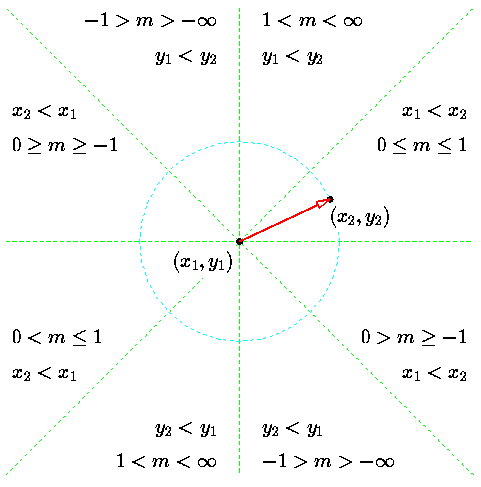
\includegraphics[height=5.5cm]{img/octants.png}
	\caption{The 8 octants and their slopes \cite{mallinus}.}
	\label{fig:octants}
\end{figure}

Let's say we have plotted a pixel $(x,y)$ of the rasterised line. Because of the constraint in \eqref{eq:slope_leq_1}, the next pixel can be either East ($x+1,y$) or North-East ($x+1,y+1$). When the line is drawn in 2D, for each step from $x$ to $x+1$, we have to find whether $y$ or $y+1$ is closest to the $y$ (floating) of the line. To do that, we increment $y$ by the slope $m$ (def'n of slope) and have to determine whether $y+m$ is above or below the midway $y+0.5$  between $y, \ y+1$ (Fig. \ref{fig:grid_line_1st_octant}).

\begin{multicols}{2}
	\begin{figure}[H]
		\centering
		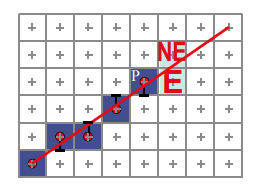
\includegraphics[height=4cm]{img/next_pixel_n_ne.png}
		\caption{At every update of pixel $(x,y)$, we choose between the E and NE neighbour \cite{mdamian}.}
		\label{fig:}
	\end{figure}
\columnbreak
	\begin{figure}[H]
	\centering
	

%\usepackage{tikz}
\usetikzlibrary{calc}


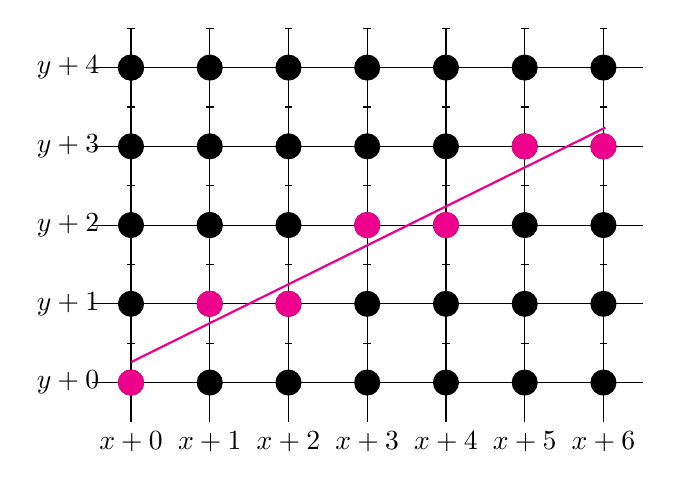
\begin{tikzpicture}
	\begin{scope}
		
\tikzset{dot/.style={fill=black,circle}}

%\foreach\l[count=\y] in {E,...,A}
\foreach \y in {0,1,...,4}
{
\draw (0.5,\y+1) -- (7.5,\y+1);
\node at (0.2,\y+1){$y + \y$};
}

\foreach \x in {0,1,...,6}
{
\draw (\x+1,0.5) -- (\x+1,5.5);
\node at (\x+1, 0.25){$x + \x$};
}

\foreach \x in {1,2,...,7}
{
	\foreach \y in {1,2,...,5}
	{
		\node[dot] at (\x,\y){};
		\draw(\x-0.05,\y+0.5) --(\x+0.05,\y+0.5);
	}
}


\node(p1)[dot] at (1,5){};
\node(p2)[dot] at (2,3){};

% the actual line
\node(st) at (0.88,1.2){};
\node(end) at (7.15,4.3){};
\draw [magenta, thick] (st) -- (end);

% draw its Bresenham points
\node[dot,magenta] at (1,1){};
\node[dot,magenta] at (2,2){};
\node[dot,magenta] at (3,2){};
\node[dot,magenta] at (4,3){};
\node[dot,magenta] at (5,3){};
\node[dot,magenta] at (6,4){};
\node[dot,magenta] at (7,4){};

	\end{scope}
\end{tikzpicture}

	\caption{The nodes represent pixel centres and the segments the midway $y$ between neighbouring pixels. Nodes in magenta represent where the line will be drawn in the 2D discrete space.}
	\label{fig:grid_line_1st_octant}
\end{figure}


\end{multicols}

\subsubsection{Bresenham's line drawing at 1st octant; the derivation}

Because we plot the original line in a discrete grid given a resolution, it will almost never cross a discrete point. Therefore it will always be at some error $\epsilon$ above or below the nearest discrete $y$. For the error \cite{mallinus},
\begin{equation}
	-0.5 \leq \epsilon <0.5
\end{equation}
The $y_{actual}$ ordinate of the line is then given by $y_{actual} = y+\epsilon$. In moving from $x$ to $x+1$ we increase the value of the true (mathematical) $y$-ordinate by an amount equal to the slope $m$ (Fig. \ref{fig:error_diagram}).
\begin{figure}[H]
	\centering
	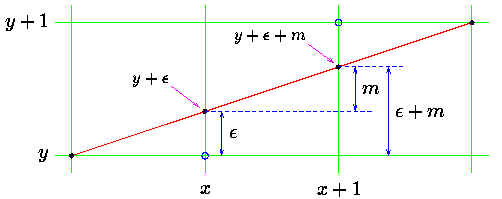
\includegraphics[height=4.5cm]{img/error_diagram.png}
	\caption{The error at each pixel during the update \cite{mallinus}.}
	\label{fig:error_diagram}
\end{figure}
From the plot in Fig. \ref{fig:error_diagram}, it is clear after the transition $x\rightarrow x+1$, if 
\begin{gather*}
	y + \epsilon + m < y+  0.5 \Rightarrow\\
	\epsilon + m < 0.5
\end{gather*}
, then we move East ($x+1,y$) to represent the line. Else we move North-East ($x+1,y+1$). We make this decision to minimise the total error between what gets drawn on the display and the actual values.

However, after $x\rightarrow x+1$ the error gets updated too from $\epsilon$ to $\epsilon_{new}$. We know that the error the distance of the mathematical line to the nearest $y$-ordinate of the grid, i.e. either $y$ or $y+1$. In case $(x+1,y)$, the new error is given by \cite{mallinus} (Fig. \ref{fig:error_diagram})
\begin{equation}
	\epsilon_{new} \leftarrow (y+\epsilon + m) - y  = \epsilon + m
\end{equation}
Else, if ($x+1,y+1$) was chosen
\begin{equation}
	\epsilon_{new} \leftarrow (y+\epsilon + m) - (y+1) = \epsilon + m -1	
\end{equation}
Therefore a first implementation of the line drawing algorithm so far is below. Note that it still uses floating point which must be eliminated. Note also that for the algorithm to be consistent with the idea developed thus far, it is assumed that $(x_1,y_1)$ is closer to the origin than $(x_2,y_2)$.
\begin{algorithm}[H]
\caption{Line drawing with FP operations.}
\label{alg:line_drawing_fp}
\begin{algorithmic}[1]
\Procedure{Line-Drawing-FP} {$x_1,\; y_1,\; x_2,\; y_2$} 
	\State $m \leftarrow \frac{y_2-y_1}{x_2-x_1} $
	\State $\epsilon \leftarrow 0, \; y\leftarrow y_1$ \Comment{$\epsilon, \; y$ are all we keep track of.}
\For{$x=x_1,\ldots,x_2$} 
	\State DrawPixel($x,\; y$)
	\If{$\epsilon + m < 0.5$}
		\State $\epsilon \leftarrow \epsilon + m$ \Comment{Move E; don't change $y$}
	\Else
		\State $\epsilon \leftarrow \epsilon + m - 1$ \Comment{Move NE}
		\State $y\leftarrow y + 1$
	\EndIf
\EndFor
\EndProcedure
\end{algorithmic}
\end{algorithm}
\marginnote{Bresenham relies on integer operations.}To optimise the algorithm, we must convert the following to integer operations
\begin{gather*}
\epsilon + m < 0.5 \tag{1}	\\
	\epsilon \leftarrow \epsilon + m \tag{2}\\
	\epsilon \leftarrow \epsilon + m - 1 \tag{3}
\end{gather*}
Plugging in $m=\Delta x/\Delta y = (y_2-y_1)/(x_2-x_1)$, Eq. (1) becomes
\[	
	2\underbrace{\epsilon\Delta x}_{\epsilon'}  + 2\Delta y < \Delta x \tag{1'}
\]
Eq. (2) and (3) become respectively
\begin{gather*}
	\underbrace{\epsilon\Delta x}_{\epsilon'} \leftarrow \underbrace{\epsilon \Delta x}_{\epsilon'} + \Delta y \tag{2'}\\
	\underbrace{\epsilon\Delta x}_{\epsilon'} \leftarrow \underbrace{\epsilon \Delta x}_{\epsilon'} + \Delta y - \Delta x \tag{3'}\\
\end{gather*}
\marginnote{Algo stated assuming $0\leq m \leq 1$ and $x_1<x_2$.}.The quantity $\epsilon\Delta x$ appears in all Eq. (1'), (2'), (3') therefore we let $\epsilon' := \epsilon \Delta x$. The algorithm we have arrived in is \textit{Bresenham's for the 1st octant}. It is written in integer arithmetic as follows:
\begin{algorithm}[H]
\caption{Bresenham's line drawing -- 1st octant.}
\label{alg:bres_1st_oct}
\begin{algorithmic}[1]
\Procedure{Bresenham-1st-Octant} {$x_1,\; y_1,\; x_2,\; y_2$} 
	\State $\Delta x \leftarrow x_2 - x_1$
	\State $\Delta y \leftarrow y_2 - y_1$
	\State $\epsilon' \leftarrow 0, \; y\leftarrow y_1$ \Comment{$\epsilon', \; y$ are all we keep track of.}
	\If {$0 \leq \frac{\Delta y}{\Delta x} < 1 $}
\For{$x=x_1,\ldots,x_2$} 
	\State DrawPixel($x,\; y$)
	\If{$2(\epsilon'  + \Delta y) < \Delta x$}
		\State $\epsilon' \leftarrow \epsilon' + \Delta y$ \Comment{Move E; don't change $y$}
	\Else
		\State $\epsilon' \leftarrow \epsilon' + \Delta y - \Delta x$ \Comment{Move NE}
		\State $y\leftarrow y + 1$
	\EndIf
\EndFor
\EndIf
\EndProcedure
\end{algorithmic}
\end{algorithm}
This version is particularly efficient not only due to integer arithmetic but as multiplication by 2 can be implemented as left bit shifting. We can of course move the update $\epsilon' \leftarrow \epsilon'+\Delta y$ before the if-else block to end up with only one if for slightly more conciseness. 


\subsubsection{Bresenham's line drawing algorithm in octant 2}

We now address the case of drawing a line with slope $1 \leq m < \infty$, i.e. one that spans at the 2nd octant (Fig. \ref{fig:octants}). Note that a line $(l1): \; y=mx+b$ with slope $0 \leq m < 1$ in the first octant is symmetric w.r.t to $y=x$ to the line $(l2): \; x=my+b \Leftrightarrow y = \frac{x}{m} - \frac{b}{m}$ (e.g. Fig. \ref{fig:symmetric_lines_octants_1_2}). If $(x_0,y_0)\in(l1)$ then $(y_0,x_0)\in (l2)$. Therefore to rasterise $(l2)$ we can apply Alg. \ref{alg:bres_1st_oct} on it modified by swapping $x$ with $y$ and $\Delta x$ with $\Delta y$. Don't forget the ordinate condition for the 2nd octant, which is $y_1<y_2$.
\begin{figure}[H]
	\centering
	\usetikzlibrary{calc}


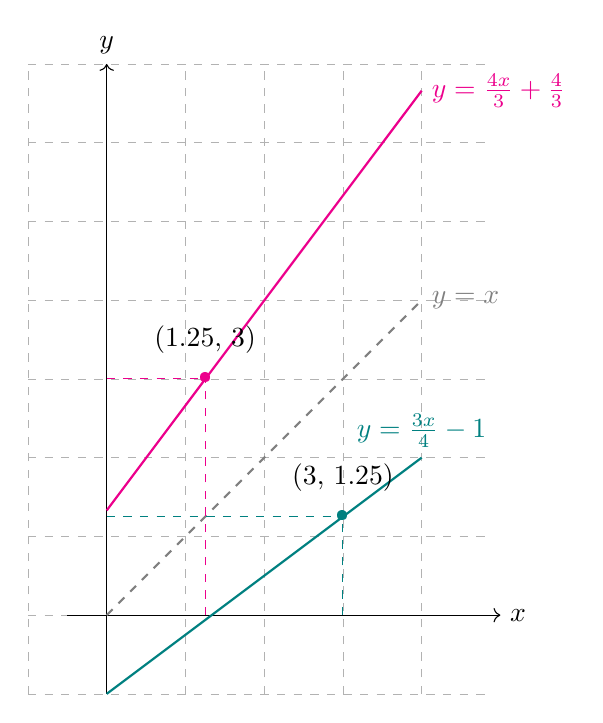
\begin{tikzpicture}
	\begin{scope}
\draw[help lines, color=gray!60, dashed] (-1,-1) grid (4.9,7);
\draw[->] (-0.5,0)--(5,0) node[right]{$x$};
\draw[->] (0,-1)--(0,7) node[above]{$y$};
\draw[thick,teal] (0,-1)--(4,2) node[above]{$y=\frac{3x}{4}-1$};
\draw[thick,magenta] (0,1.33)--(4,6.66) node[right]{$y= \frac{4x}{3}+ \frac{4}{3}$};
\draw[thick,gray,dashed] (0,0)--(4,4) node[right]{$y=x$};

\node [magenta, label={(1.25,$\ $3)}] at (1.25,3) {\textbullet};
\node [teal, label={(3,$\ $1.25)}] at (3, 1.25) {\textbullet};

\draw[thick,thin,teal,dashed] (3,0)--(3,1.25) node[right]{};
\draw[thick,thin,teal,dashed] (0,1.25)--(3,1.25) node[right]{};

\draw[thick,thin,magenta,dashed] (1.25,0)--(1.25,3) node[right]{};
\draw[thick,thin,magenta,dashed] (0,3)--(1.25,3) node[right]{};

	\end{scope}
\end{tikzpicture}

	\caption{Two lines in the first two octants symmetric about line $y=x$.}
	\label{fig:symmetric_lines_octants_1_2}
\end{figure}
\begin{algorithm}[H]
\caption{Bresenham's line drawing -- 2nd octant.}
\label{alg:bres_2nd_oct}
\begin{algorithmic}[1]
\Procedure{Bresenham-2nd-Octant} {$x_1,\; y_1,\; x_2,\; y_2$} 
	\State $\Delta x \leftarrow x_2 - x_1$
	\State $\Delta y \leftarrow y_2 - y_1$
	\State $\epsilon' \leftarrow 0, \; x\leftarrow x_1$ \Comment{$\epsilon', \; y$ are all we keep track of.}
	\If {$1\leq \frac{\Delta y}{\Delta x} $ and $y_1<y_2$}
		\For{$y=y_1,\ldots,y_2$} 
			\State DrawPixel($x,\; y$)
			\If{$2(\epsilon'  + \Delta x) < \Delta y$}
				\State $\epsilon' \leftarrow \epsilon' + \Delta x$ 
			\Else
				\State $\epsilon' \leftarrow \epsilon' + \Delta x - \Delta y$ 
				\State $x\leftarrow x + 1$
			\EndIf
		\EndFor
	\EndIf
\EndProcedure
\end{algorithmic}
\end{algorithm}
Octants 1 and 2 (quadrant 1) have been addressed. To complete the algorithm in the remaining 6 octants, observe that quadrant 2 (octants 3,4) is symmetric with quadrant 1 w.r.t the $y$ axis. Quadrant 3 (octants 5, 6) is symmetric with 1 w.r.t $x$ and $y$ axes, and quadrant 4 is symmetric with 1 w.r.t the $x$ axis.


\subsubsection{Bresenham's line drawing algorithm in octants 3 and 4}

Octants 3 and 4 are symmetric w.r.t the $y$ axis to octants 2 and 1 respectively. Therefore to derive their line drawing we start with Alg. \ref{alg:bres_2nd_oct} and \ref{alg:bres_1st_oct} respectively and substitute $(-x,y) \leftarrow (x,y)$, $\Delta x \leftarrow -\Delta x$. Therefore the line drawing for those octants is formulated as follows, renaming the error $\epsilon'$ to $\epsilon$ for simplicity.
\begin{algorithm}[H]
\caption{Bresenham's line drawing -- 2nd quadrant.}
\label{alg:bres_2nd_qd}
\begin{algorithmic}[1]
\Procedure{Bresenham-2nd-Quadrant} {$x_1,\; y_1,\; x_2,\; y_2$} 
	\State $\Delta x \leftarrow x_2 - x_1$
	\State $\Delta y \leftarrow y_2 - y_1$
	\State $\epsilon \leftarrow 0, \; y\leftarrow y_1$ 
	\If {$\frac{\Delta y}{\Delta x} < -1$ and $y_1 < y_2$} \Comment{This is the 3rd octant (2nd octant mirror w.r.t $y$ axis)}
		\For{$y=y_1,\ldots,y_2$} 
			\State DrawPixel($x,\; y$)
			\If{$2(\epsilon  - \Delta x) < \Delta y$}
				\State $\epsilon \leftarrow \epsilon - \Delta x$ 
			\Else
				\State $\epsilon \leftarrow \epsilon - \Delta x - \Delta y$ 
				\State $x\leftarrow x - 1$
			\EndIf
		\EndFor
	\ElsIf {$0 \leq \frac{\Delta y}{\Delta x} < -1 $ and $x_2 < x_1$} \Comment{4th octant (1st octant mirrored w.r.t $y$ axis)}
			
		\For{$x=x_1,\ldots,x_2$} 
			\State DrawPixel($x,\; y$)
			\If{$2(\epsilon  + \Delta y) < -\Delta x$}
				\State $\epsilon \leftarrow \epsilon + \Delta y$
			\Else
				\State $\epsilon \leftarrow \epsilon + \Delta y + \Delta x$ 
				\State $y\leftarrow y + 1$
			\EndIf
	    \EndFor	
	\EndIf
\EndProcedure
\end{algorithmic}
\end{algorithm}
In the same way, given the algorithm for the first two octants, using the transform $(x,y) \leftarrow (-x,-y), \; \Delta x \leftarrow -\Delta x$, $\Delta y \leftarrow -\Delta y$ we can derive octants 5 and 6. Finally, using $(x,y) \leftarrow (x,-y), \; \Delta y \leftarrow -\Delta y$ we can derive octants 7 and 8. The $x$'s, $y$'s, $\Delta x$'s and $\Delta y$'s for each octant given the first are summarised in Fig. \ref{fig:all_octants_x_y}.

\begin{figure}[H]
	\centering
	\makeatletter
\newsavebox{\measure@tikzpicture}
\NewEnviron{scaletikzpicturetowidth}[1]{%
  \def\tikz@width{#1}%
  \def\tikzscale{1}\begin{lrbox}{\measure@tikzpicture}%
  \BODY
  \end{lrbox}%
  \pgfmathparse{#1/\wd\measure@tikzpicture}%
  \edef\tikzscale{\pgfmathresult}%
  \BODY
}

\begin{scaletikzpicturetowidth}{0.4\textwidth}
\begin{tikzpicture}[scale=\tikzscale]
\draw[help lines, color=gray!30, dashed] (-4.9,-4.9) grid (4.9,4.9);
\draw[->,thick] (-5,0)--(5,0) node[right]{$x$};
\draw[->, thick] (0,-5)--(0,5) node[above]{$y$};
\draw [ultra thin, dashed, color=black!50](0,0) circle (4cm);

\draw[magenta,thick] (-4,-4)--(4,4) node[above]{$y=x$};
\draw[magenta,thick] (4,-4)--(-4,4) node[above]{$y=-x$};
\node[text width=2cm,align=right] at (2,1) {$(x,y)$, $(\Delta x, \Delta y)$};
\node[text width=2cm,align=right] at (1,3.5) {$(y,x)$, $(\Delta y, \Delta x)$};
\node[text width=2cm,align=right] at (-2,3.5) {$(-y,x)$, $(-\Delta y, \Delta x)$};
\node[text width=2cm,align=right] at (-3.5,1) {$(-x,y)$, $(-\Delta x, \Delta y)$};

\node[text width=2cm,align=right] at (-3.5,-1) {$(-x,-y)$, $(-\Delta x, -\Delta y)$};
\node[text width=2cm,align=right] at (-2,-3.5) {$(-y,-x)$, $(-\Delta y, -\Delta x)$};
\node[text width=2cm,align=right] at (2,-1) {$(x,-x)$, $(\Delta x, -\Delta y)$};
\node[text width=2cm,align=right] at (1,-3.5) {$(y,-x)$, $(\Delta y, -\Delta x)$};

\end{tikzpicture}

\end{scaletikzpicturetowidth}

	\caption{The Bresenham signs for the full circle given the 1st octant.}
	\label{fig:all_octants_x_y}
\end{figure}


\subsection{Bresenham's line drawing generalisation and implementation}

The first step of the algorithm generalisation is to determine the octant of the line, which is done with the aid of the conditions in Fig. \ref{fig:octants}. Next, we start from the algorithm for quadrants 1 and 2 and transform the $x$'s, $y$'s, $\Delta x$'s and $\Delta y$'s given the symmetry . The pseudocode for the full algorithm is listed in \ref{app:bresenham_full_p}.

To implement Bresenham and draw pixels in C, Prof D. Thain's ``gfx'' graphics library \cite{thain} was used. Method \texttt{gfx\_line\_bres} was added to implement the algorithm. To test it, each line was plotted against the library's \texttt{gfx\_line} method and the lines overlapped for all 8 octants. The code for the full algorithm in C is found in \ref{app:bresenham_full_src}.

Finally, note that the algorithm runs in linear ($\mathcal{O}(n)$) time.


\subsection{Summary -- pros and cons}
Bresenham's algorithm may be easy to implement and fast, but has a certain disadvantage. However it is still used by graphics cards and software libraries \cite{bhowmick} thanks to its simplicity.

Pros:
\begin{itemize}
	\item Simple to implement, can be efficiently implemented practically on any hardware!
	\item Fast -- linear time.
\end{itemize}
Cons:
\begin{itemize}
	\item Does not account for aliasing.
\end{itemize}


\clearpage
\section{Triangle fill algorithms}

There are various algorithms to draw a solid triangle. Here, we discuss three of them:
\begin{enumerate}
    \item Line sweep (row-by-row fill).
    \item Triangle interior test
    \item Bresenham-based fill.
\end{enumerate}

\subsection{Line sweep triangle fill}

Suppose we want to fill a triangle given points $P_1=(x_1,y_1)$, $P_2=(x_2,y_2)$, $P_3=(x_3,y_3)$, $y_1 \geq y_2 \geq y_3$. Line sweep fill fills the interior points of the triangle row by row relying on the fact that the slope of each line $P_1P_2$ and $P_2P_3$ is constant.

At each iteration, it keeps track of three variables -- the row number ($y$ coordinate), the leftmost ordinate (column) of the line to draw ($x_l$), and  the rightmost ordinate (column) of the line to draw ($x_r$). At each row sweep, we incrementally update $x_l$ and $x_r$. Then, we can fill all pixels from $x_l$ to $x_r$, forming a horizontal line (a.k.a. scanline). Finally, because the slope changes as we move from line $P_1P_2$ to $P_2P_3$, we first draw the top flat triangle $\Updelta(P_1P_2P_2')$ and then the $\Updelta(P_2'P_2P_3)$. 

\begin{figure}[H]
    \centering
    \subfloat[\centering Triangle fill variables.]{{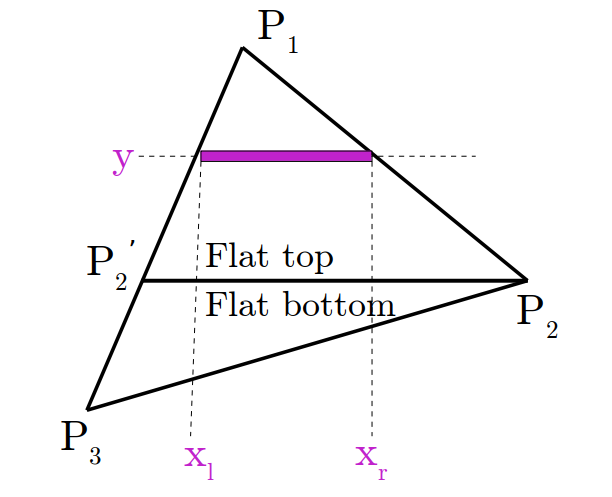
\includegraphics[width=4.75cm]{img/triangle_fill_variables.png} }}%
    \qquad
    \subfloat[\centering Angles $a_1,a_2,a_3$ are utilised by the algorithm. highlighted.]{{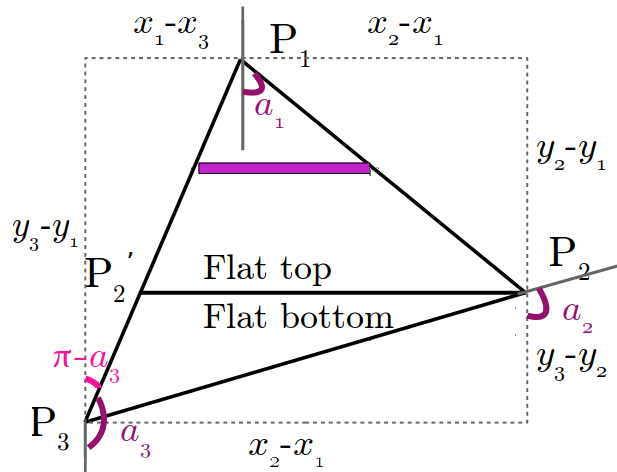
\includegraphics[width=4.75cm]{img/triangle_fill_variables_angles.png} }}%
    \caption{Line sweep fill divides the original triangle in two flat ones. (a) The variables $y,x_l,x_r$ considered at each iteration. (b) The angles utilised by the algorithm to update $x_l$, $x_r$}%
    \label{fig:triangle_line_sweep_vars}%
\end{figure}

What's left to define is how $x_l$ and $x_r$ are updated at each iteration. Because $x$ is a function of $y$ (we iterated row-by-row), we increment the $y$ of each line by the \textit{inverse slope} (i.s.) of that line. The inverse slope has $x$ as the adjacent side and $y$ as the opposite, therefore $m_{inv} = \tfrac{\Delta x}{\Delta y}$. $x_l$ is always incremented by the inverse slope of line $\overline{P_1P_3}$ and $x_r$ is incremented by the i.s. of whatever line it belongs it; by $m_{inv,13}$ is if $y \leq y_2$, else by $m_{inv,23}$. The i.s. $m_{inv,13}$ of $\overline{P_1P_1}$ is the tangent of $a_3$ (Fig. \ref{fig:triangle_line_sweep_vars}):
\[
m_{inv,13} = \tan{a_3} = -\tan(\pi - a_3) = -\frac{x_1-x_3}{y_3-y_1} = \frac{x_3-x_1}{y_3-y_1}
\]
\begin{align*}
\therefore
    m_{inv,13} = \frac{x_3-x_1}{y_3-y_1}\\
    m_{inv,12} = \frac{x_2-x_1}{y_2-y_1}\\
    m_{inv,23} = \frac{x_3-x_2}{y_3-y_2}
\end{align*} 
The formulas would end up the same if $P_2$ was left of $P_3$. The final algorithm, which fills $\Updelta (P_1P_2P_2\prime)$ first, followed by $\Updelta ( P_2\prime P_2P_3)$ is listed below.

\begin{algorithm}[H]
\caption{Triangle fill by line sweep pseudocode.}
\begin{algorithmic}[1]
\Procedure{TriangleFillLineSweep} {$x_1,\ y_1,\ x_2,\ y_3,\ x_3,\ y_3$} \Comment{Assuming $y_1 < y_2 < y_3$}
    \State $m_{inv,13} \leftarrow \frac{x3-x_1}{y_3 - y_1}$
    \State $m_{inv,12} \leftarrow \frac{x2-x_1}{y_2 - y_1}$
    \State $m_{inv,23} \leftarrow \frac{x3-x_2}{y_3 - y_2}$
    \State $x_l \leftarrow x_1$
    \State $x_r \leftarrow x_1$
    \For{$y=y_1.\ .\ y_2$} \Comment{Flat top triangle}
        \For{$y=\textup{int}(x_l).\ .\ \textup{int}(x_r)$} \Comment{int denotes the casting from float to int}
            \State drawPixel($x,y$)
        \EndFor
        \State $x_l \leftarrow x_l + m_{inv,13}$
        \State $x_r \leftarrow x_r + m_{inv,12}$
    \EndFor
    \For{$y=y_2.\ .\ y_3$} \Comment{Flat bottom}
        \For{$y=\textup{int}(x_l).\ .\ \textup{int}(x_r)$}
            \State drawPixel($x,y$)
        \EndFor
        \State $x_l \leftarrow x_l +  m_{inv,13}$
        \State $x_r \leftarrow x_r +  m_{inv,23}$
    \EndFor
\EndProcedure
\end{algorithmic}
\label{alg:triangle_fill_line_sweep}
\end{algorithm}
This is super easy to implement and an implementation in C is found in my ``gfx-v4'' repository at \url{https://github.com/0xLeo/gfx-v4/blob/master/src/gfx/gfx.c#L395}.

% https://www.cs.princeton.edu/courses/archive/spring05/cos426/lectures/09-scan.pdf



\subsection{Triangle fill by interior test}


\subsubsection{Mathematical background}
Another method to fill the interior of a triangle is to find its bounding box, scan row-by-row all pixels in the box, and determine whether each pixel is in the interior of the triangle. The only tricky part about this algorithm is to derive an ``interior test''.

Before delving in the algorithm or in its maths, we need the definition of \emphasis{perpendicular } vector (a.k.a. \emphasis{perp}) in 2D.
\begin{definition}[perp vector]
Given a vector $\ba = (a_x, a_y)$, its \emphasis{perp vector} $\ba^{\bot}$ is defined as a vector with the same magnitude rotated by $90\degree$ ccw:
\begin{equation}
\ba^{\bot} = (-a_y, a_x)
\end{equation}
\end{definition}
\begin{figure}[H]
    % ref isbn 0-12-336155-9 p. 138
    \centering
    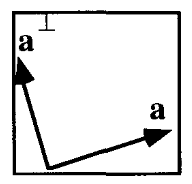
\includegraphics[height=2cm]{img/vec_perp.png}
    \caption{Vector $\ba$ and its ``perp'' ($\ba$) rotated by $90\degree$ ccw.}
\end{figure}

The perp vector comes in handy when we want to determine the relative orientation of two vectors, e.g. whether $\ba$ is cw or ccw from $\textbf{b}$. But first, it's imortant to clarify what is meant by cw and ccw. By saying that $\bb$ is cw of $\ba$, it is implied that to rotate $\bb$ by the \textit{inner} (smaller) angle until it's aligned with $\ba$, we move clockwise. Ccw rotation is defined in the same way. The figure below illustrates this.

\begin{figure}[H]
    \centering
    \subfloat[\centering $\bb$ cw from $\ba$]{{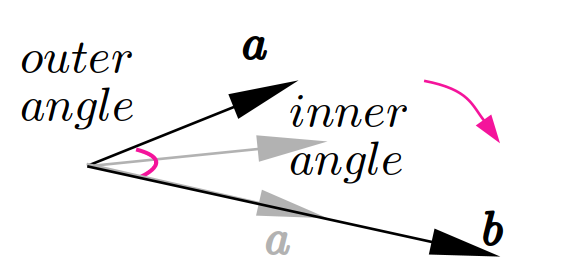
\includegraphics[height=2.25cm]{img/b_cw_from_a.png} }}%
    \qquad
    \subfloat[\centering $\bb$ ccw from $\ba$]{{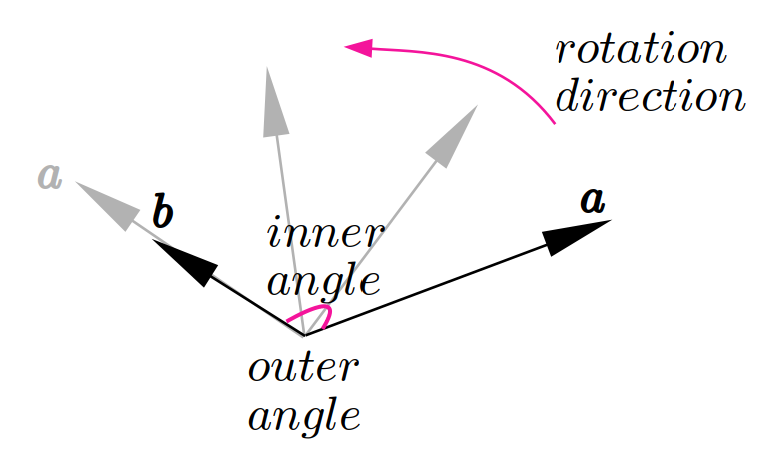
\includegraphics[height=3cm]{img/b_ccw_from_a.png} }}%
    \caption{cw and ccw terminology}%
    \label{fig:cw_ccw_terms}%
\end{figure}

Back to the perp vector, how is it able to tell us the relative orientation between $\ba$ and $\bb$? Remember that $\bb^{\bot}$ is $\bb$ rotated by $90\degree$ ccw. It turns out that if $\bb$
 is ccw from $\ba$, then $\ba^{\bot}\bb = \norm{\ba}\norm{\bb}\cos(\theta) < 0$, since $\theta > 90\degree$ (Fig. \ref{fig:b_ccw_a_sign_pdot}).
 
\begin{figure}[H]
    \centering
    \subfloat[\centering $\ba^{\bot}\bb <0$ when $b$ is ccw from $\ba$ and the angle between $\ba$, $\bb$ is obtuse.]{{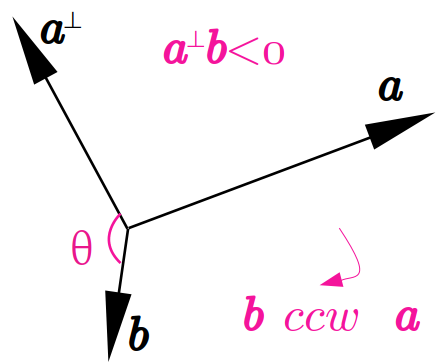
\includegraphics[height=2.5cm]{img/a_perpdot_b_ccw_obtuse.png} }}%
    \qquad
    \subfloat[\centering $\ba^{\bot}\bb <0$ when $b$ is ccw from $\ba$ and the angle between $\ba$, $\bb$ is acute.]{{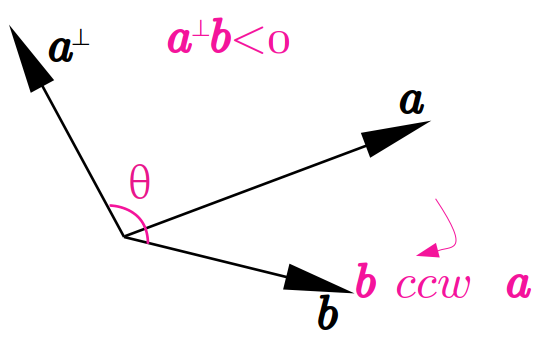
\includegraphics[height=2.5cm]{img/a_perpdot_b_ccw_acute.png} }}%
    \caption{$\ba^{\bot}\bb <0$ when $\bb$ is ccw is $\ba$.}%
    \label{fig:b_ccw_a_sign_pdot}%
\end{figure}

Similarly, when $\bb$ is cw from $\ba$ then $\ba$, then $\ba^{\bot}\bb = \norm{\ba}\norm{\bb}\cos(\theta) > 0$, since $\theta < 90\degree$ (Fig. \ref{fig:b_ccw_a_sign_pdot}).

\begin{figure}[H]
    \centering
    \subfloat[\centering $\ba^{\bot}\bb >0$ when $b$ is cw from $\ba$ and the angle between $\ba$, $\bb$ is obtuse.]{{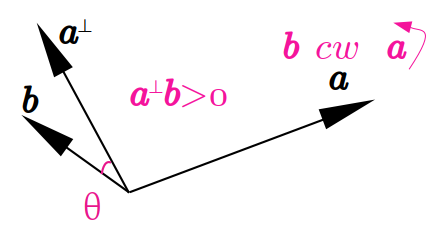
\includegraphics[height=2cm]{img/a_perpdot_b_cw_obtuse.png} }}%
    \qquad
    \subfloat[\centering $\ba^{\bot}\bb >0$ when $b$ is cw from $\ba$ and the angle between $\ba$, $\bb$ is acute.]{{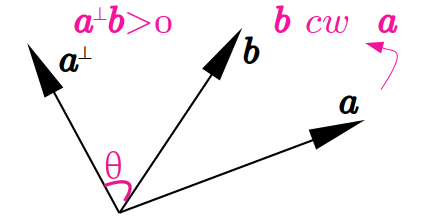
\includegraphics[height=2cm]{img/a_perpdot_b_cw_acute.png} }}%
    \caption{$\ba^{\bot}\bb <0$ when $\bb$ is ccw is $\ba$.}%
    \label{fig:b_cw_a_sign_pdot}%
\end{figure}

Therefore the so-called ``perp dot product'' tells us the relative orientation between $\ba$ and $\bb$. To define it:

\begin{definition}[perp dot product]
The \emphasis{perp dot product} between $\ba$ and $\bb$ is defined as:
\begin{equation}
    pdot(\ba, \bb) = \ba ^{\bot} \bb  = 
    a_xb_y - a_yb_x
    \left|
    \begin{matrix}
    a_x & a_y \\
    b_x & b_y
    \end{matrix}
    \right |
\end{equation}
, where $\ba^{\bot}$ is $\ba$ rotated by $90\degree$, i.e. $\ba^{\bot} = \begin{bmatrix}
0 & -1 \\-1 & 0\end{bmatrix}\ba$.
\end{definition}
To summarise, it has the following properties:
\begin{corollary}[properties perp product]
\label{cor:prop_pdot_prod}
\begin{gather}
    \ba^{\bot} \bb > 0 \quad \textup{if} \quad \bb \quad \textup{ccw} \quad \textup{from} \quad \ba \label{eq:prop_pdot_ccw}\\
    \ba^{\bot} \bb < 0 \quad \textup{if} \quad \bb \quad \textup{cw} \quad \textup{from} \quad \ba \label{eq:prop_pdot_cw}
    \\
    \ba^{\bot} \bb = 0 \quad \textup{if} \quad \bb = \lambda \ba, \quad \lambda \in \setR
    \label{eq:prop_pdot_par}
\end{gather}
\end{corollary}


\subsubsection{Stating the interior test}

Using Cor. \ref{cor:prop_pdot_prod}, we can formulate whether a 2D point $P$ is inside or outside a triangle $\Updelta(P_1P_2P_3)$. We can use the perp dot product of vectors  $\overrightarrow{PP_1}$, $\overrightarrow{PP_2}$, and $\overrightarrow{PP_3}$ to deduce whether $P$ is inside or outside of the triangle, given that we know the relative orientation of points $P_1, P_2, P_3$, i.e. of vectors $\overrightarrow{OP_1}, \overrightarrow{OP_2},\overrightarrow{OP_3}$, where $O$ is the origin. To reiterate, We make two assumptions:
\begin{enumerate}
    \item $y_1 \leq y_2 \leq y_3$
    \item About the relative orientation of points $P_1, P_2, P_3$; they are either in cw or ccw.
\end{enumerate}

The figures below show the vectors $\overrightarrow{PP_1}$, $\overrightarrow{PP_2}$, and $\overrightarrow{PP_3}$ for the ccw and cw cases.

\begin{figure}[H]
    \centering
    \subfloat[\centering Vectors connecting $P$ and $Q$ to the vertices  when $P_1, P_2, P_3$ are ccw.]{{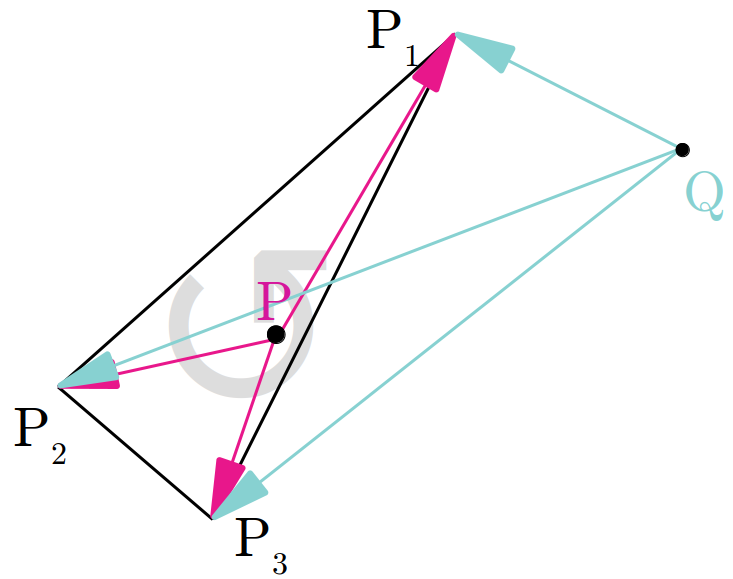
\includegraphics[height=3.2cm]{img/triangle_int_ext_ccw.png} }}%
    \qquad \qquad
    \subfloat[\centering Vectors connecting $P$ and $Q$ to the vertices  when $P_1, P_2, P_3$ are cw.]{{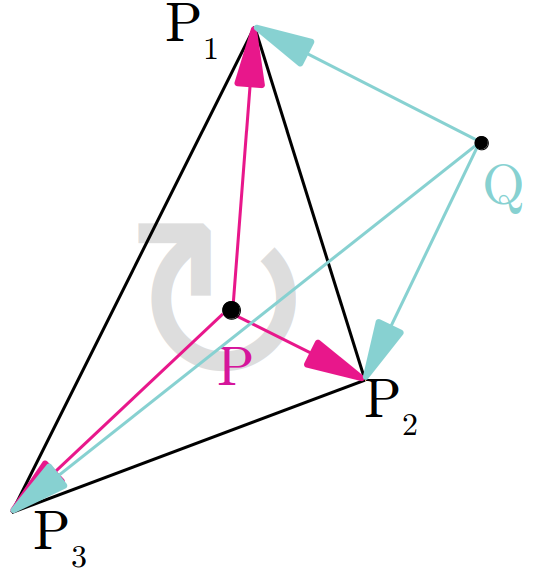
\includegraphics[height=3.2cm]{img/triangle_int_ext_cw.png} }}%
    \caption{For the interior test, we consider the vectors from a point to the vertices. The vectors for a typical interior point  $P$ and an exterior point $Q$ are drawn.}
    \label{fig:triangle_int_ext}
\end{figure}

From \eqref{eq:prop_pdot_cw}, \eqref{eq:prop_pdot_ccw} and Fig. \ref{fig:triangle_int_ext} we can see that in case $P_1,P_2,P_3$ are ccw, then for an interior point (e.g. $P$):
\begin{align*}
    \overrightarrow{PP_2} \quad \textup{ccw} \quad \textup{from} \quad \overrightarrow{PP_1} \Rightarrow \overrightarrow{PP_1}^{\bot}\overrightarrow{PP_2} > 0 \tag{1} \\
    \overrightarrow{PP_3} \quad \textup{ccw} \quad \textup{from} \quad \overrightarrow{PP_2} \Rightarrow \overrightarrow{PP_2}^{\bot}\overrightarrow{PP_3} > 0 \tag{2} \\
    \overrightarrow{PP_1} \quad \textup{ccw} \quad \textup{from} \quad \overrightarrow{PP_3} \Rightarrow \overrightarrow{PP_3}^{\bot}\overrightarrow{PP_1} > 0 \tag{3}
\end{align*}
Similarly, from the same figure and equations  for the cw case we obtain:
\begin{align*}
    \overrightarrow{PP_2} \quad \textup{cw} \quad \textup{from} \quad \overrightarrow{PP_1} \Rightarrow \overrightarrow{PP_1}^{\bot}\overrightarrow{PP_2} < 0 \tag{4} \\
    \overrightarrow{PP_3} \quad \textup{cw} \quad \textup{from} \quad \overrightarrow{PP_2} \Rightarrow \overrightarrow{PP_2}^{\bot}\overrightarrow{PP_3} < 0 \tag{5} \\
    \overrightarrow{PP_1} \quad \textup{cw} \quad \textup{from} \quad \overrightarrow{PP_3} \Rightarrow \overrightarrow{PP_3}^{\bot}\overrightarrow{PP_1} <  \tag{6}0
\end{align*}
, where $\overrightarrow{PP_i} = \overrightarrow{OP_i} - \overrightarrow{OP}$. To summarise, an interior point satisfies either Eq. (1) and Eq. (2) and Eq. (3) or Eq. (4) and Eq. (5) and Eq. (6). Otherwise, it's exterior. We can therefore state the interior test in pseudocode as follows.
\begin{algorithm}[H]
\caption{Testing whether a point $P(x,y)$ lies in the interior of a triangle $\Updelta(P_1P_2P_3)$.}
\begin{algorithmic}[1]
\Procedure{PerdDotProd}{$x_1,y_1,x_2,y_2$}
\State \textbf{return} $x_1y_2 - y_1x2$
\State
\EndProcedure
\Procedure{IsInterior} {$x_1,y_1,x_2,y_2,x_3,y_3,x,y$}
\State $PP1_x \leftarrow x - x_1$ \Comment{vector from $P(x,y)$ to verices $P_i(x_i,y_i)$}
\State $PP1_y \leftarrow y - y_1$
\State $PP2_x \leftarrow x - x_2$
\State $PP2_y \leftarrow y - y_2$
\State $PP3_x \leftarrow x - x_3$
\State $PP3_y \leftarrow y - y_3$
\State cw $\leftarrow$ PerdDotProd$(PP1_x,PP1_y,PP2_x,PP2_y) < 0$ AND

\quad PerdDotProd$(PP2_x,PP2_y,PP3_x,PP3_y) < 0$ AND

\quad PerdDotProd$(PP3_x,PP3_y,PP1_x,PP1_y) < 0$
\State ccw$\leftarrow$ PerdDotProd$(PP1_x,PP1_y,PP2_x,PP2_y) > 0$ AND 

\quad PerdDotProd$(PP2_x,PP2_y,PP3_x,PP3_y) > 0$ AND

\quad PerdDotProd$(PP3_x,PP3_y,PP1_x,PP1_y) > 0$
\State \textbf{return} cw OR ccw \Comment{cw and ccw are boolean type}
\EndProcedure
\end{algorithmic}
\label{alg:triangle_fill_int_test}
\end{algorithm}

\subsubsection{The algorithm}

As usual, the aim of the algorithm is to fill a triangle given 3 points $P_1, P_2, P_3$, assuming $y_1\leq y_2 \leq y_3$. We can then iterate over every pixel of the bounding box of the triangle (see Fig. \ref{fig:triangle_line_sweep_vars}) and apply the interior test (Alg. \ref{alg:triangle_fill_int_test}) to each. Below is the basic pseudocode, without any cache misses/ hits considered.

\begin{algorithm}[H]
\caption{Triangle fill by interior test (see Alg. \ref{alg:triangle_fill_int_test} for interior test).}
\begin{algorithmic}[1]
\Procedure{TriangleFillInteriorTest} {$x_1,y_1,x_2,y_2,x_3,y_3$} \Comment{Assuming $y_1\leq y_2 \leq y_3$}
\State xmin $\leftarrow \min(x_1,x_2,x_3)$
\State xmax $\leftarrow \max(x_1,x_2,x_3)$
\For{x$\leftarrow$ xmin $. \ . \ $ xmax}
\For{y$\leftarrow y_1. \ . \ y3$}
\If{IsInterior(x,y)} putPixel(x,y)
\EndIf
\EndFor
\EndFor
\EndProcedure
\end{algorithmic}
\end{algorithm}
This algorithm completely avoids floating point operations, unlike Alg. \ref{alg:triangle_fill_line_sweep} (triangle fill by line sweep). In my ``gfx-v4'' repo, it is implemented in \url{https://github.com/0xLeo/gfx-v4/blob/master/src/gfx/gfx.c#L444}.
% https://blackpawn.com/texts/pointinpoly/#:~:text=Same%20Side%20Technique,triangle%2C%20otherwise%20it%20is%20not.
% http://www.sunshine2k.de/coding/java/PointInTriangle/PointInTriangle.html#perpdotproduct
% https://courses.cs.washington.edu/courses/cse457/06au/lectures/triangle_intersection.pdf
% https://stackoverflow.com/questions/2049582/how-to-determine-if-a-point-is-in-a-2d-triangle

% implementation tips:
% https://stackoverflow.com/a/30982985



\clearpage
\section{Circle rasterisation (midpoint algorithm)}

\subsection{Derivation of the algorithm}
One way to draw a circle centred at $(0,0)$ is by plotting the two $y$'s given by the circle equation for each $x$.  
\begin{align*}
x^2+y^2=r^2 \Rightarrow \\
y = \pm \sqrt{r^2 - x^2}
\end{align*}
However, this method has two drawbacks; the square root is very expensive and the line is not guaranteed to be continuous, especially when the slope is high.

The goal is to derive an algorithm that plots a continuous circle using cheap operations. We can exploit the 8--way symmetry of a circle about its centre to derive the algorithm for one octant and then derive the rest, as illustrated in Fig. \ref{fig:all_octants_x_y}. 

For the sake of convention, we will start with octant 2, i.e. starting from $x=0,\ y=r$ and incrementing $x$ until $y=x$, therefore for the slope $m$: $0 \leq m \leq 1$. Because we work in octant 2 (going clockwise), assuming we have just plotted pixel $(x_p,y_p)$, we can either move to $E(x_p+1, y_p)$ or $SE(x_p+1, y_p-1)$ (Fig. \ref{fig:bres_algo_next_pixel}). Which of the two to select though? The idea is that if the circle curve passes above the midpoint $M(x_p+1, y_p-\tfrac{1}{2})$ of the next two choices, then we select $E(x_p+1, y_p)$. Otherwise, we select $SE(x_p+1, y_p-1)$.

\begin{figure}[H]
    \centering
    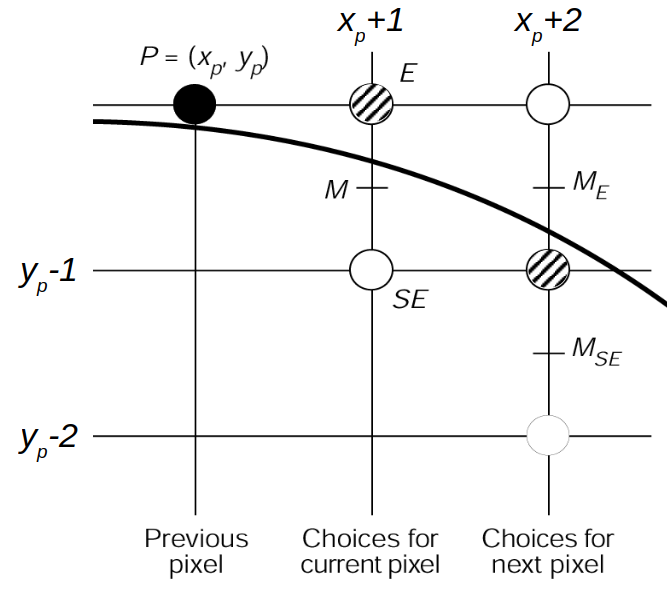
\includegraphics[height=3.25cm]{img/bres_algo_next_pixel.png}
    \caption{The two possible choices for the next pixel when drawing a circle at octant 2; E and SE. For the above curve, we select E and SE as the next two pixels (striped).}
    \label{fig:bres_algo_next_pixel}
\end{figure}

We need a decision variable to determine which pixel to visit next (E or SE). The midpoint $M$ between S and SE is at distance $(x_p+1)^2 + (y_p - \tfrac{1}{2})^2$ from the origin. As shown in Fig. \ref{fig:bres_algo_next_pixel}:
\begin{itemize}
    \item If $r^2 \geq (x_p+1)^2 + (y_p - \tfrac{1}{2})^2$, then we choose to visit the E pixel as it's closer to the line.
    \item Otherwise SE is closer and we visit this one.
\end{itemize}
Therefore we define the decision variable w.r.t. the midpoint $M(x_p+1, y_p-\tfrac{1}{2})$ as:
\begin{align*}
    D &= F(M) = F\Bigg(x_p+1, y_p-\frac{1}{2}\Bigg)\\
    &= (x_p+1)^2 + (y_p-\frac{1}{2})^2 - r^2
\end{align*}
And we decide:
\begin{itemize}
    \item If $D\geq 0$, the next pixel is SE.
    \item If $D<0$, the next pixel is E.
\end{itemize}
It's important to note that at each iteration we compute the current $D$ given the previous. Therefore we need to define how we accumulate it in case E or SE was chosen next.
\begin{itemize}
    \item In case $E(x_p+1, y_p-\tfrac{1}{2})$ was chosen, then the new midpoint (at $x_p+1+1$) is $M(x_p+2, y_p-\frac{1}{2})$. Then it can be proven (App. \ref{app:decision_var_update}) that the new value of the decision variable is:
    \begin{equation}
    D_{E} = D + (2x_p + 3)
    \label{eq:de}
    \end{equation}
    Hence, $D$ is incremented by $2x_p + 3$.
    \item In case $SE(x_p+1, y_p-1-\tfrac{1}{2})$ was chosen, then the new midpoint is also $M(x_p+2, y_p-\frac{1}{2})$ -- same as before. Then it can be proven (App. \ref{app:decision_var_update}) that the decision variable $D$ is incremented by $2x_p-2y_p+5$:
    \begin{equation}
        D_{SE} = D + (2x_p-2y_p+5)    
        \label{eq:d_se}
    \end{equation}
    
\end{itemize}
All that's left to define is how to initialise $D$. Because we start at $(0, r)$ going clockwise, the first midpoint is at $M(1, r - \tfrac{1}{2})$. Therefore the initial decision variable is:
\begin{align*}
    D_0 &= F(1, r-\frac{1}{2}) \\
    &= 1 + (r-\frac{1}{2})^2  - r^2 \\
    &= 1+ r^2 - r + \frac{1}{4} - r^2\\
    &= \frac{5}{4} - r  
\end{align*}
To avoid dealing with floating points ($\tfrac{5}{4}$), notice that on each iteration we compare $D$ to 0. $D$ also gets updated with an integer quantity -- either $2x_p+3$ or $2x_p-2y_p+5$. Therefore $D+\tfrac{1}{4}$ is positive only when $D$ is positive; it is safe to drop the $\tfrac{1}{4}$. Hence, we can set $D_0$ to $1-r$ instead.
\begin{equation}
    D_0 = 1-r
    \label{eq:d_0}
\end{equation}
Using the update rules in \eqref{eq:de}, \eqref{eq:d_se}, \eqref{eq:d_0}, we can draw a circular arc on the 2nd octant and mirror it on the rest to draw a full circle.

% https://www.cs.bgu.ac.il/~graph161/wiki.files/09c-Rasterization.pdf
% https://www.cs.bgu.ac.il/~graph161/wiki.files/09c-Rasterization.pdf
% https://en.wikipedia.org/wiki/Midpoint_circle_algorithm
% http://clux.x-pec.com/files/mathstuff/4thyear/CS324%20Computer%20Graphics/bres2.pdf
% https://weber.itn.liu.se/~stegu/circle/circlealgorithm.pdf
% https://stackoverflow.com/questions/33526137/where-am-i-going-wrong-in-bresenham-circle-drawing-algorithm
% https://www.ques10.com/p/22016/explain-mid-point-circle-generation-algorithm-in-d/
% file:///tmp/4221.pdf



\subsection{Pseudocode and implementation of the algorithm}

% ref https://www.ques10.com/p/22016/explain-mid-point-circle-generation-algorithm-in-d/
\begin{algorithm}[H]
\caption{Midpoint algorithm for circle drawing at a point $(x_0,y_0)$ with radius $r$.}
\begin{algorithmic}[1]
\Procedure{MidpointAlgorithm} {$x_0,y_0,r$}
\State $x \leftarrow 0$
\State $y \leftarrow r$
\State $D \leftarrow 1 - r$ \Comment{Decision variable}
\Do
    \State putPixel($x + x_0,\ y + y_0$)    \Comment{Octant 2; draw all octants to fill the circle}
    \State putPixel($y + x_0,\ x + y_0$)    \Comment{Octant 1}
    \State putPixel($-x + x_0,\ y + y_0$)    \Comment{Octant 3}
    \State putPixel($-y + x_0,\ x + y_0$)    \Comment{Octant 4}
    \State putPixel($-y + x_0,\ -x + y_0$)    \Comment{Octant 5}
    \State putPixel($-x + x_0,\ -x + y_0$)    \Comment{Octant 6}
    \State putPixel($x + x_0,\ -y + y_0$)    \Comment{Octant 7}
    \State putPixel($y + x_0,\ -x + y_0$)    \Comment{Octant 8}
    \If{$D<0$}
        \State $D\leftarrow D + 2x + 3$
    \Else
        \State $y\leftarrow y - 1$
        \State $D \leftarrow D + 2x - 2y + 5$
    \EndIf  
    \State $x \leftarrow x + 1$
\doWhile{$x < y$} % <--- use \doWhile for the "while" at the end
\EndProcedure
\end{algorithmic}
\end{algorithm}
An implementation in C is found in my ``gfx-v4'' repo at \url{https://github.com/0xLeo/gfx-v4/blob/master/src/gfx/gfx.c#L355}.

%=-=-=-=-=-=-=-=-=-=-=-=-=-=-=-=-=-=-=-=-=-=-=-=-=-=-=-=-=-=-=-=-=-=-=-=-=-=-=-=-
% References
%=-=-=-=-=-=-=-=-=-=-=-=-=-=-=-=-=-=-=-=-=-=-=-=-=-=-=-=-=-=-=-=-=-=-=-=-=-=-=-=-
\newpage
\printbibliography



%=-=-=-=-=-=-=-=-=-=-=-=-=-=-=-=-=-=-=-=-=-=-=-=-=-=-=-=-=-=-=-=-=-=-=-=-=-=-=-=-
% Appendices
%=-=-=-=-=-=-=-=-=-=-=-=-=-=-=-=-=-=-=-=-=-=-=-=-=-=-=-=-=-=-=-=-=-=-=-=-=-=-=-=-
\newpage
\appendix

\section{Appendices}

% ------------------------ New appendix ------------------------ %

\subsection{Bresenham's straight line drawing algorithm -- pseudocode}
\label{app:bresenham_full_pseudo}

\begin{algorithm}[H]
\caption{Bresenham's full line drawing.}
\label{alg:bres_pt2}
\begin{algorithmic}[1]
	\Procedure{Find-Octant} {$x_1,y_1,x_2,y_2$} \Comment{See Fig. \ref{fig:octants}}
	\State $m \leftarrow \frac{y_2-y_1}{x_2-x_1}$
	\If {$x_1 \leq x_2$ and $0\leq m \leq 1$}
		\State \textbf{return} 0 \Comment{1st}
	\ElsIf {$y_1 \leq y_2$ and $ m > 1$}
		\State \textbf{return} 1 \Comment{etc.}
	\ElsIf {$y_1 \leq y_2$ and $ m < -1 $}
		\State \textbf{return} 2
	\ElsIf {$x_2 \leq x_1$ and $0 \geq m \geq -1$}
		\State \textbf{return} 3
	\ElsIf {$x_2 \leq  x_1$ and $0 < m \leq 1$}
		\State \textbf{return} 4
	\ElsIf {$y_2 \leq  y_1$ and $ m > 1$}
		\State \textbf{return} 5
	\ElsIf {$y_2 \leq y_1$ and $ m < -1$}
		\State \textbf{return} 6
	\ElsIf {$x_1 \leq x_2$ and $-1 \leq m \leq 0$}
		\State \textbf{return} 7
	\Else \Comment{$x_1 = x_2$, vertical line}
		\State \textbf{return} 8
	\EndIf
\EndProcedure
\State
\Procedure{Bresenham} {$x_1,\; y_1,\; x_2,\; y_2$} 
	\State $\Delta x \leftarrow x_2 - x_1$
	\State $\Delta y \leftarrow y_2 - y_1$
	\State $\epsilon \leftarrow 0$
	\State $oct \leftarrow$ Find-Octant($x1,y1,x2,y2$)
	\If {$oct = 0$} \Comment{0 to 45 degrees with $x$ axis}
		\State $y \leftarrow y_1$
		\For {$x=x1..x2$}
			\State Draw-Pixel($x,y$)
			\State $\epsilon \leftarrow \epsilon + \Delta y$
			\If {$2\epsilon \geq \Delta x$}
				\State $\epsilon \leftarrow \epsilon - \Delta x$
				\State $y \leftarrow y + 1$
			\EndIf
		\EndFor
	\ElsIf {$oct = 1$} \Comment{45 to 90}
		\State $x \leftarrow x_1$
		\For {$y = y_1..y_2$}
			\State Draw-Pixel($x,y$)
			\State $\epsilon \leftarrow \epsilon + \Delta x$
			\If {$2\epsilon \geq \Delta y$}
				\State $\epsilon \leftarrow - \Delta y$
				\State $x \leftarrow x + 1$
			\EndIf
		\EndFor
	\ElsIf {$oct = 2$} \Comment{90 to 135}
		\State $x \leftarrow x_1$
		\For {$y=y_1..y_2$}
			\State Draw-Pixel($x,y$)
			\State $\epsilon \leftarrow \epsilon - \Delta x$
			\If { $2\epsilon \geq \Delta$}
				\State $\epsilon \leftarrow \epsilon - \Delta y$
				\State $x \leftarrow x - 1$
			\EndIf
		\EndFor
	\ElsIf {$oct = 3$}  \Comment{135 to 180}
		\State $y \leftarrow y_1$
		\For {$x=x_1..x_2$}
			\State Draw-Pixel($x,y$)

		\EndFor
	\EndIf
\EndProcedure
\end{algorithmic}
\end{algorithm}


\begin{algorithm}[H]
\caption{Bresenham's full line drawing -- cont'ed}
\label{alg:bres_pt2}
\begin{algorithmic}[1]
	\Indent
	\State $\epsilon \leftarrow \epsilon + \Delta x$
	\If {$2\epsilon \geq - \Delta x$}
		\State $\epsilon \leftarrow \epsilon + \Delta x$
		\State $y \leftarrow y + 1$
	\ElsIf {$oct = 4$}  \Comment{180 to 215}
		\State $y\leftarrow y_1$
		\For { $x=x_1..x_2$}
			\State Draw-Pixel($x,y$)
			\State $\epsilon \leftarrow \epsilon - \Delta y$
			\If {$2\epsilon \geq -\Delta x$}
				\State $\epsilon \leftarrow \epsilon + \Delta x$
				\State $y \leftarrow y - 1$
			\EndIf
		\EndFor
	\ElsIf {$oct = 5$} \Comment{215 to 270}
		\State $x\leftarrow x_1$
		\For {$y=y_1..y_2$}
			\State Draw-Pixel($x,y$)
			\State $\epsilon \leftarrow \epsilon - \Delta x$
			\If {$2\epsilon \geq - \Delta y$}
				\State $\epsilon \leftarrow \epsilon - \Delta y$
				\State $x \leftarrow x - 1$
			\EndIf
		\EndFor
	\ElsIf {$oct = 6$} \Comment{270 to 315}
		\State $x = x_1$
		\For {$y=y_1..y_2$}
			\State Draw-Pixel($x,y$)
			\State $\epsilon \leftarrow \epsilon + \Delta x$
			\If {$2\epsilon \geq -\Delta y$}
				\State $\epsilon \leftarrow \epsilon + \Delta y$
				\State $x\leftarrow x+1$
			\EndIf
		\EndFor
	\ElsIf {$oct = 7$} \Comment{315 to 360}
		\State $x\leftarrow x_1$
		\For {$y=y_1..y_2$}
			\State Draw-Pixel($x,y$)
			\State $\epsilon \leftarrow \epsilon + \Delta x$
			\If {$2\epsilon \geq -\Delta y$}
				\State $\epsilon \leftarrow \epsilon + \Delta y$
				\State $x\leftarrow x+ 1$
			\EndIf
		\EndFor
	\ElsIf {$oct = 8$} \Comment{Vertical line}
	\State \Comment{Draw a vertical at line at $x_1$ between $y1,\; y_2$}
	\EndIf
	\EndIndent
\end{algorithmic}
\end{algorithm}


\newpage
\subsection{Bresenham's line drawing source code in C}
\label{app:bresenham_full_src}

From \url{https://github.com/0xLeo/gfx-v4}.
\lstinputlisting[language=C,caption={Bresenham's code (\detokenize{src/bresenham.c)}.}, label=src:mylabel]{src/bresenham.c}



%---------------------------------------- new appendix ----------------------------------------
\newpage
\subsection{Midpoint algorithm -- decision variable update}
\label{app:decision_var_update}
In case $E(x_p+2, y_p-\frac{1}{2})$ was chosen as the next point, then the new decision variable variable is:
\begin{align*}
    D_E &= F(x_p + 2, y_p - \frac{1}{2}) \\
        &= (x_p+2)^2 + (y_p - \frac{1}{2})^2 - r^2 \\
        &= (x_p^2+4x_p+2) + (y_p-\frac{1}{2})^2 - r^2 \\
        &= (x_p +2x_p + 1) + (2x_p + 3) + (y_p-\frac{1}{2})^2 - r^2 \\
        &= (x_p+1)^2 + (y_p-\frac{1}{2})^2 -r^2 + (2x_p + 3) \\
        &= D + (2x_p+3)
\end{align*}
In case $SE(x_p+2, y_p-1-\frac{1}{2})$ was chosen as the next point, then the new decision variable variable is:
\begin{align*}
    D_{SE} &= F(x_p+2, y_p -\frac{3}{2}) \\
    &= (x_p+2)^2 + (y_p-\frac{3}{2})^2 \\
    &= (x_p^2 + 2x_p + 1) + (2x_p+3) + (y_p^2 -y_p + \frac{1}{4}) + (-2y_p+\frac{8}{4}) - r^2 \\
    &= (x_p+1)^2 + (y_p - \frac{1}{2})^2 - r^2 + (2x_p+3) + (-2y_p + 2) \\
    &= D + (2x_p -2y_p + 5)
\end{align*}

\end{document}